\section{} \label{appendix:a}

% code and images go here
\subsection{Subsystem Requirements and Verification Tables} \label{appendix:a:subsystemreqs}

\subsubsection{Control Unit}
\begin{table}[ht]
    \centering
    \caption{Control Unit Subsystem Requirements and Verification}
    \begin{tabular}{p{0.45\linewidth}p{0.45\linewidth}}
    \toprule
    \textbf{Requirements} & \textbf{Verification} \\
    \midrule
    \begin{itemize}[leftmargin=*, nosep, after=\strut]
        \item Must be able to communicate with the sensors and LEDs through the PCB
        \begin{itemize}[nosep]
            \item Must be able to output 4.8±0.3V to the LEDs
            \item The accelerometer must be able to detect acceleration within ±1m/s.
            \item The magnetometer must be able to detect North.
            \item The gyroscope must be able to detect angular rate within ±15 dps.
        \end{itemize}
        \item Must be able to determine the correct turn signal from the IMU
        \item Must be able to turn on the LEDs based on the corresponding turn signal
        \begin{itemize}[nosep]
            \item Turn left: Must be able to flicker the left LED
            \item Turn right: Must be able to flicker the right LED
            \item Slow down: Must be able to turn on both LEDs
            \item Hazard: Must be able to flicker both LEDs
        \end{itemize}
    \end{itemize} &
    \begin{itemize}[leftmargin=*, nosep, after=\strut]
        \item Connect the IMU to the ESP32 such that the ESP32 can print the IMU acceleration readings from the accelerometer, gauss reading from the magnetometer, and the angular rate readings from the gyroscope. Drop 3 times (once for each x, y, z axis), and verify that the acceleration is g±5m/s. Point the IMU in different directions and verify that the gauss peaks when pointing North. Spin the IMU using a motor and verify that the angular rate readings match the dps of the motor ±20 dps.
        \item Using the IMU imitate the motion of each of the arm gestures and print out the detected turn signal using the software of the ESP32. Verify if the correct turn signal is displayed on the LED
        \item Move the IMU at a constant velocity and stop quickly (simulate a crash) and verify that the hazard signal is activated through the ESP32 software.
    \end{itemize} \\
    \bottomrule
    \end{tabular}
    \end{table}
    \newpage
\subsubsection{Power Subsystem}
\begin{table}[ht]
    \centering
    \caption{Power Subsystem Requirements and Verification}
    \begin{tabular}{p{0.45\linewidth}p{0.45\linewidth}}
    \toprule
    \textbf{Requirements} & \textbf{Verification} \\
    \midrule
    \begin{itemize}[leftmargin=*, nosep, after=\strut]
        \item Must be able to supply 3.3±0.3V to the IMUs and the ESP32
        \item Must be able to supply 4.8±0.3V to the LEDs
        \item The temperature of the battery should stay below 50 C during operation
        
    \end{itemize} &
    \begin{itemize}[leftmargin=*, nosep, after=\strut]
        \item The battery will be connected to the voltage regulator and a multimeter will be used to verify that the voltage output by one of the voltage regulators is 3.3±0.3V
        \item To use the multimeter, the positive lead will be connected to the output of the voltage regulator and the negative lead will be connected to the ground of the voltage regulator
        \item Measure the temperature using a thermometer during operation and ensure it is below 50 C
    \end{itemize} \\
    \bottomrule
    \end{tabular}
    \end{table}
    % \newpage
\subsubsection{LEDs}
    \begin{table}[ht]
        \centering
        \caption{LED Subsystem Requirements and Verification}
        \begin{tabular}{p{0.45\linewidth}p{0.45\linewidth}}
        \toprule
        \textbf{Requirements} & \textbf{Verification} \\
        \midrule
        \begin{itemize}[leftmargin=*, nosep]
            \item Must be able to turn on and off given a 4.8V input.
            \item Must be bright enough for drivers to see from 250ft.
            
        \end{itemize} &
        \begin{itemize}[leftmargin=*, nosep]
            \item Connect the LEDs in series with a switch and 4.8V power source and verify that the LEDs turn on.
            \item Walk 250 ft away from the LEDs while they are on and check that they are visible
        
        \end{itemize} \\
        \bottomrule
        \end{tabular}
        \end{table}
        \newpage
\subsubsection{Sensor Subsystem}
\begin{table}[ht]
    \centering
    \caption{Sensor Subsystem Requirements and Verification}
    \begin{tabular}{p{0.45\linewidth}p{0.45\linewidth}}
    \toprule
    \textbf{Requirements} & \textbf{Verification} \\
    \midrule
    \begin{itemize}[leftmargin=*, nosep]
        \item The accelerometer must be able to detect acceleration within ±1m/s.
        \item The magnetometer must be able to detect North.
        \item The gyroscope must be able to detect angular rate within ±15 dps.
        
        
    \end{itemize} &
    \begin{itemize}[leftmargin=*, nosep]
        \item Connect the IMU to the ESP32 such that the ESP32 can print the IMU acceleration readings from the accelerometer. Drop 3 times (once for each x, y, z, axis), and verify that the acceleration is g±5m/s
        \item Connect the IMU to the ESP32 such that the ESP32 can print the IMU gauss reading from the magnetometer. Point the IMU in different directions and verify that the gauss peaks when pointing North.
        \item Connect the IMU to the ESP32 such that the ESP32 can print the IMU angular rate readings from the gyroscope. Spin the IMU using a motor and verify that the angular rate readings match the dps of the motor ±20 dps.
        
    \end{itemize} \\
    \bottomrule
    \end{tabular}
    \end{table}
    \newpage

\subsection{Micellaneous} \label{appendix:a:code}

    \begin{figure}[ht]
        \centering
        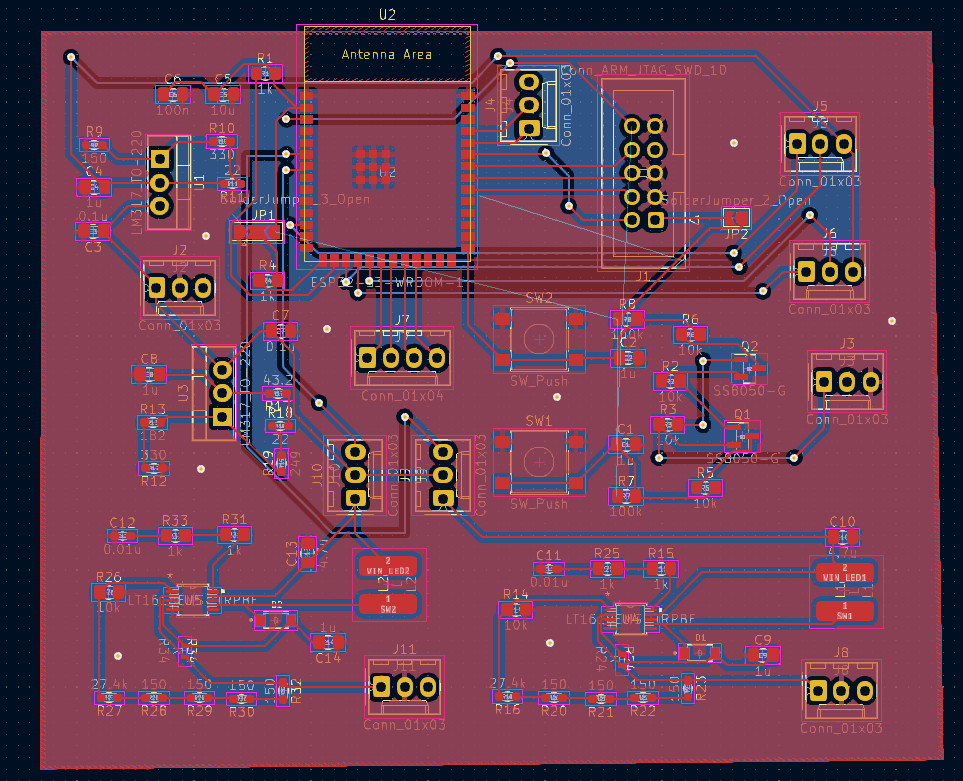
\includegraphics[width=1.0\textwidth]{images/Final_PCB.png}
        \caption{PCB layout of the final design}
        \label{fig:pcb_layout}
    \end{figure}
    
    \begin{figure}[ht]
        \centering
        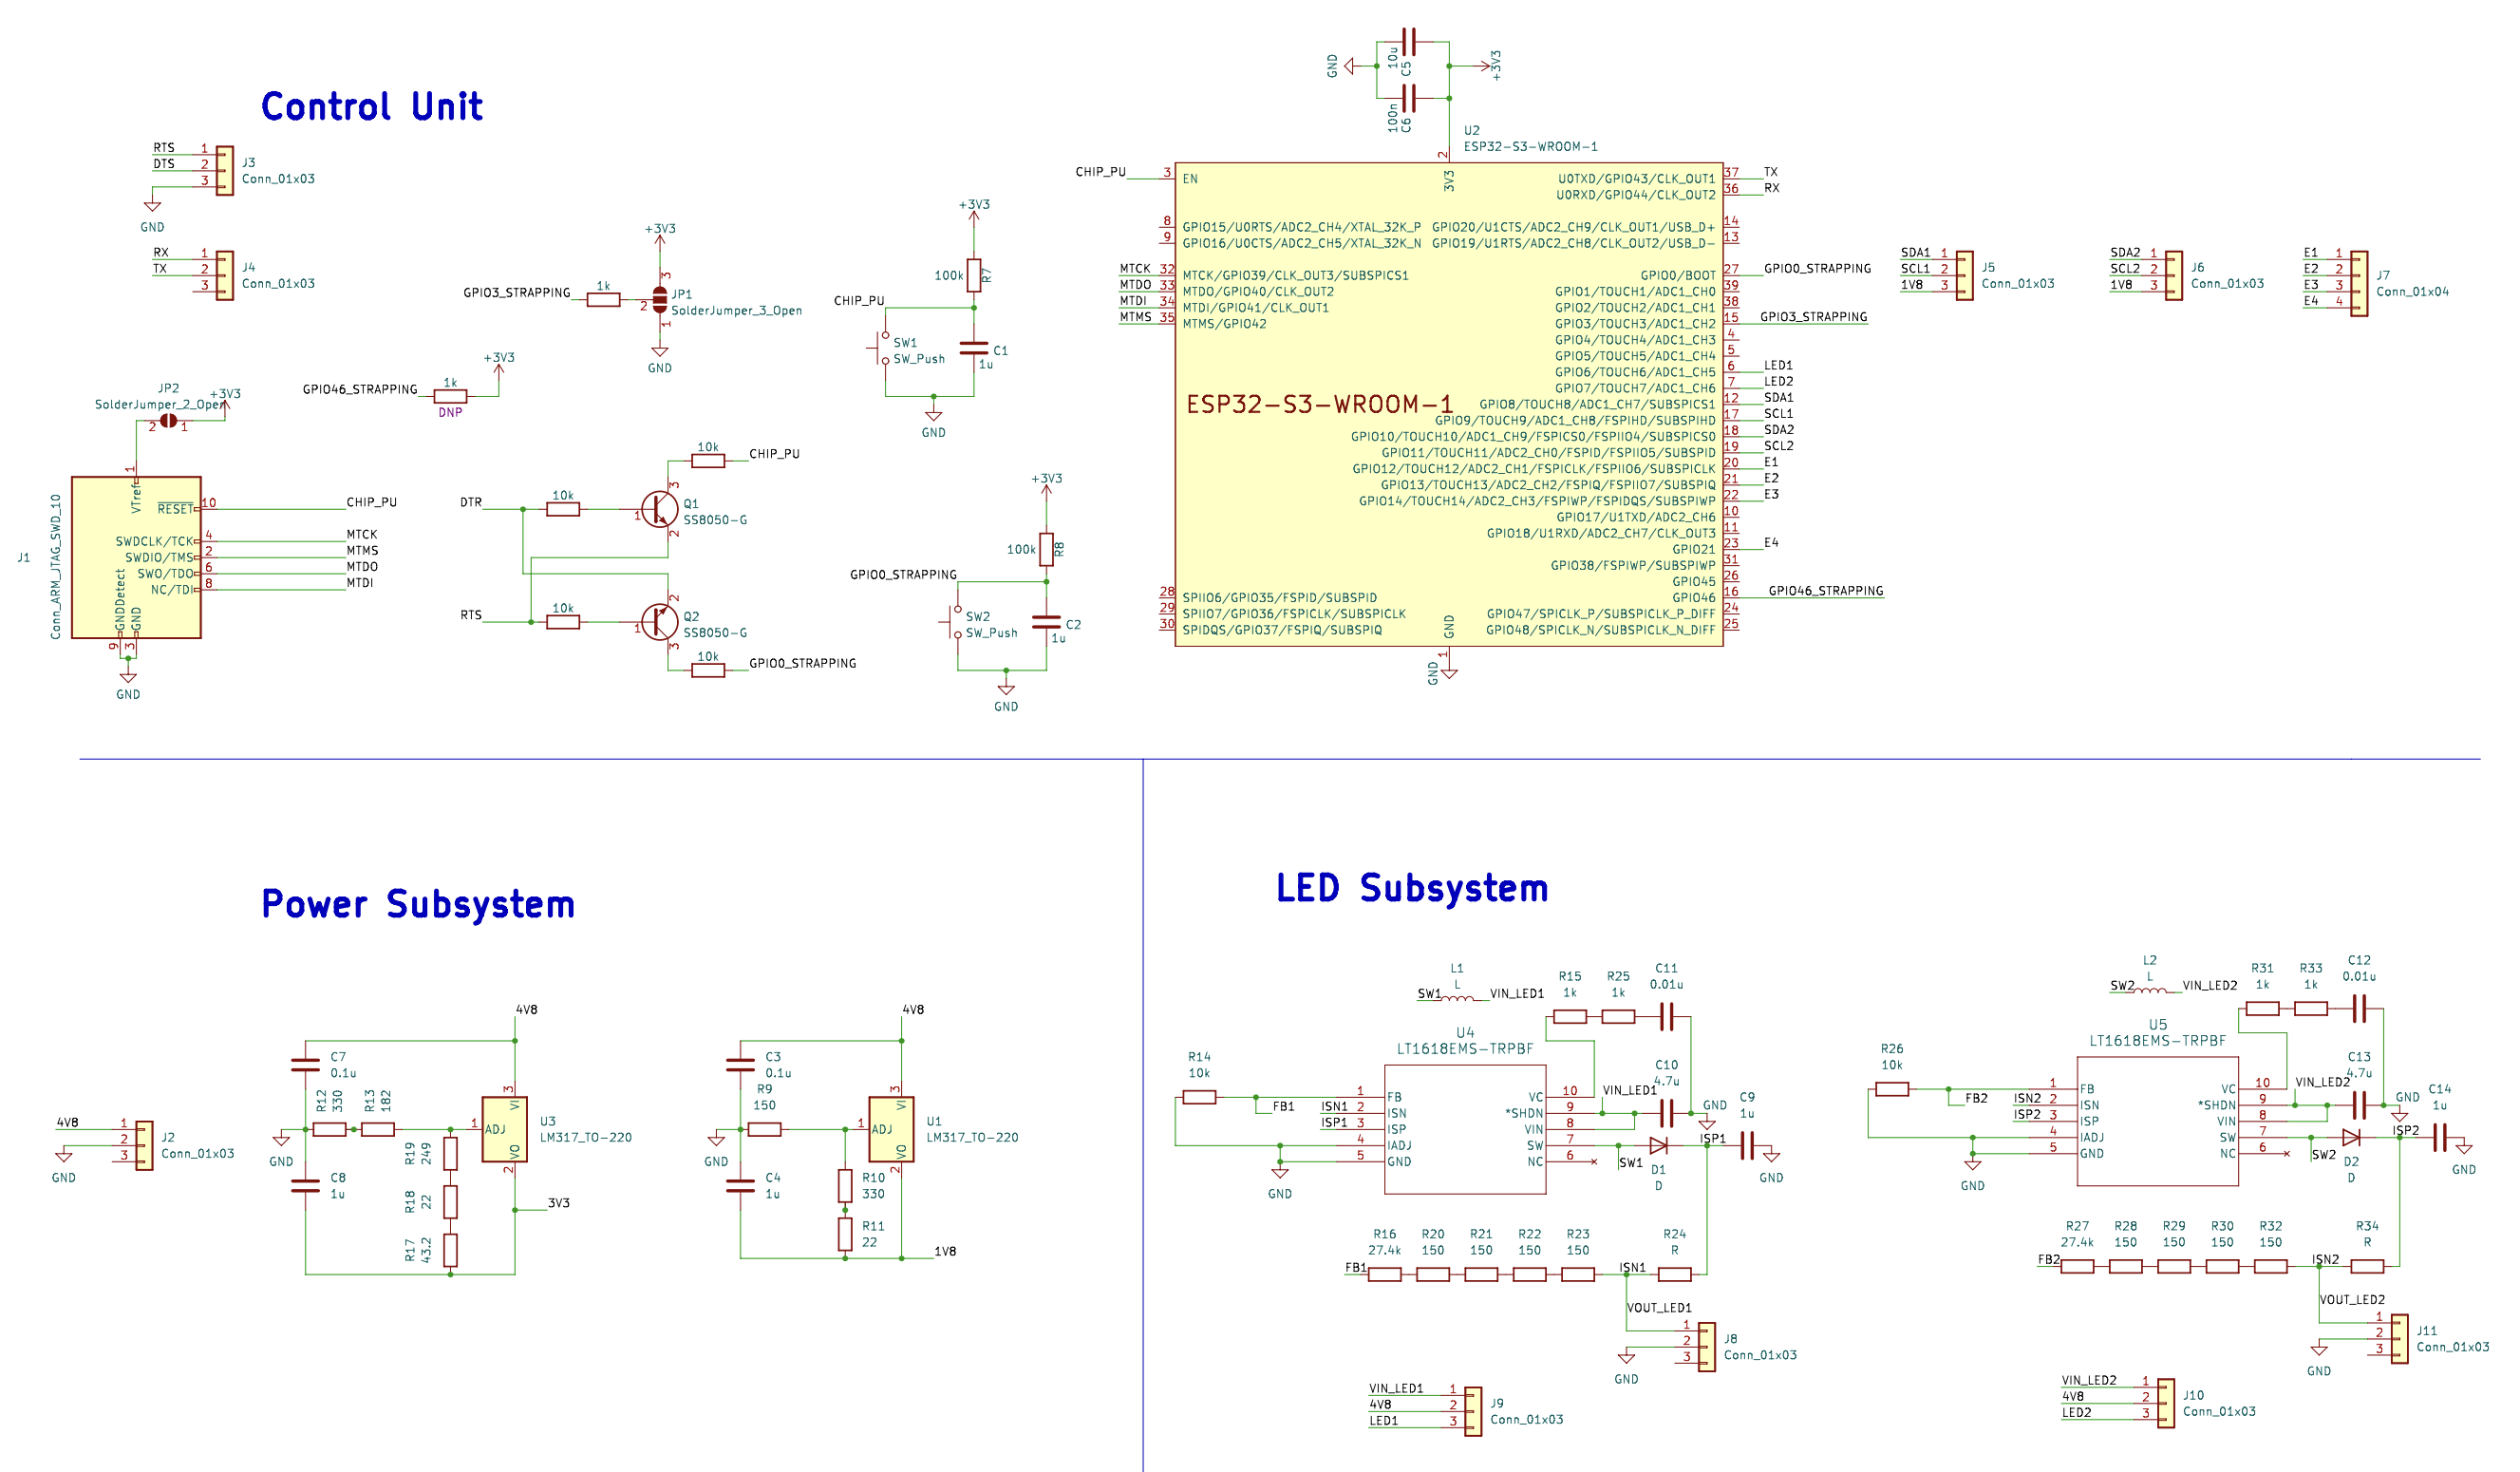
\includegraphics[width=1.0\textwidth]{images/pcb_schematic.png}
        \caption{PCB schematic of the final design}
        \label{fig:pcb_schematic}
    \end{figure}
    
    \begin{figure}[ht]
        \centering
        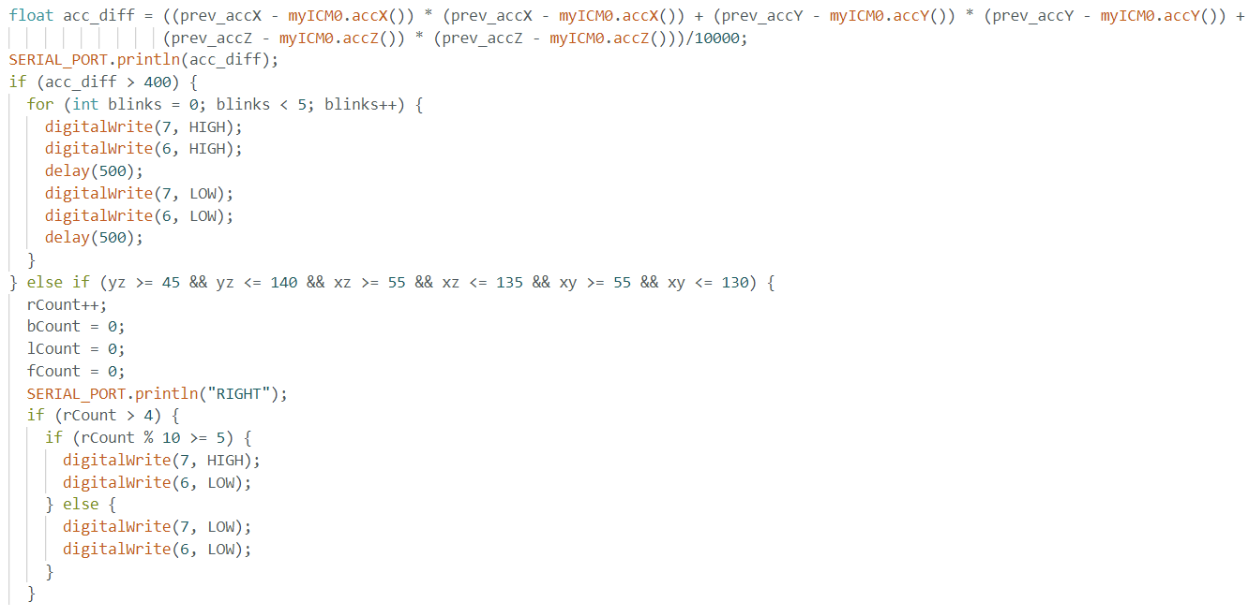
\includegraphics[width=1.0\textwidth]{images/gesture_alg.png}
        \caption{Gesture recognition algorithm}
        \label{fig:gesture_alg}
    \end{figure}
    
    \begin{figure}[ht]
        \centering
        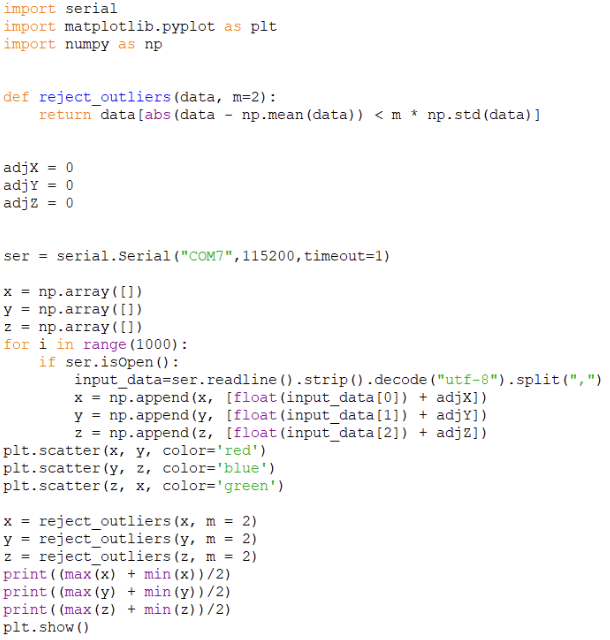
\includegraphics[width=1.0\textwidth]{images/calibration.png}
        \caption{Calibration code for magnetometers}
        \label{fig:calibration}
    \end{figure}